\section{Programs for Specific Tasks in the World of McPhase}\label{addprog}

This section  contains some further programs which do some important manipulations
in magnetism, ...
\begin{description} 

\item [\prg addj\index{addj} \addcontentsline{toc}{subsubsection}{\prg addj}
file1.j file2.j:]adds exchange parameters of file2.j to the %%@
parameters in
file1.j - output is written to stdout, if file2.j is not given, a copy of the input file is saved 

\begin{description}
\item[Option: -nofcomponents 23] fixes the nofcomponents to 23 by 
                         reducing (removing entries) or increasing (by filling with zeroes) 
                         the exchange parameter tables
\item[Option:            -ni]  forces output without indexchange 
\end{description}
\item [\prg anisotropy:]\addcontentsline{toc}{subsubsection}{\prg anisotropy} program to calculate the magnetic anistropy
by doing a mcphas or
               single ion calculation for different external magnetic field
               directions and evaluating the expectation value of the magnetic 
               moment.
\begin{verbatim}
     usage: anisotropy -h
           anisotropy  T H xn yn zn nofsteps [-r sipffilename Hxc1 Hxc2 ... Hxcnofcomponents]
           anisotropy  T H -p nofthetasteps [-r sipffilename Hxc1 Hxc2 ... Hxcnofcomponents]

     -h           : this (help) message
      T           : temperature in Kelvin
      H           : absolute value of the external magnetic field (T)
      xn,yn,zn    : direction normal to plane, in which the anisotropy
                    should be calculated ... e.g. if you want to
                    calculate the anisotropy in the xy plane, then
                    enter xn yn zn = 0 0 1
      nofsteps    : number of steps to be calculated 
     -p           : calculate polycrystal average
      nofthetastepssteps    : number of theta steps to be calculated for polycrystal average

    option:
    -r sipffilename: filename of single ion parameter file
                      Hxc1,Hxc2,... are the exchange field components (meV)
                     (exchange field is kept constant, external magnetic
                     field is rotated in the anisotropy calculation)

    output files:

    ./results/anisotropy.out  contains anisotropy information

\end{verbatim}

\item [\prg cfsplit:]\addcontentsline{toc}{subsubsection}{\prg cfsplit} Calculates via group theory, the multiplicity of crystal field split levels 
for particular point symmetries. The command is: "{\prg cfsplit $\langle$PTGP$\rangle$ $\langle$J$\rangle$}"
where {\prg $\langle$PTGP$\rangle$} is the name of the point group (both Hermman-Maguin and 
Schoenflies notation are understood), and {\prg $\langle$J$\rangle$} is the half-integer value 
of the total angular momentum J of the lowest multiplet. E.g. "{\prg cfsplit Oh 2}" gives the 
familiar cubic Eg/T2g splitting (last line of output).
See also: {\prg symhmltn} which calculates the allowed two-ion exchange terms for a point group.

\item [\prg cif2mcphas {[options]} $\langle$INPUT.CIF$\rangle$:] \addcontentsline{toc}{subsubsection}{\prg cif2mcphas}
Creates a set of McPhase input files (mcphas.j, sipfs) from the crystal structure given in a CIF 
(Crystallographic Information File), with or without user interaction. CIF input files may be obtained 
from online repositories such as the Inorganic Crystal Structures Database (ICSD), the Crystallography 
Online Database (COD) or the American Mineralogist Database (AMCSD), or they may be generated by many 
crystal structures programs, including FullProf. In fully automated mode, the program is invoked with 
the name of the CIF input file as: "{\prg cif2mcphas $\langle$INPUT.CIF$\rangle$}". In this case, the
program tries to guess which crystallographic sites contains magnetic or non-magnetic ions, and what the 
valence (oxidation state) of that ion is. This information may also be given by the user in interactive
mode, with the following command: "{\prg cif2mcphas $\langle$INPUT.CIF$\rangle$ -i}" (e.g. by including
the switch {\prg -i} (or {\prg --interactive}) before or after the CIF input filename). The online help
may be access by invoking the program without arguments or with the {\prg -h} ({\prg --help}) switch.
Finally, if you do not have a CIF of the structure you want to calculate, you can use the template here:

\begin{verbatim}
; Please replace text in square brackets [] with your data
_cell_length_a                     [a_in_Angstrom]
_cell_length_b                     [b_in_Angstrom]
_cell_length_c                     [b_in_Angstrom]
_cell_angle_alpha                  [alpha_in_degrees]
_cell_angle_beta                   [beta_in_degrees]
_cell_angle_gamma                  [gamma_in_degrees]
; The H-M symbol generally needed by cif2mcphas but some spacegroups
; which have only one setting can be identified purely by the number.
; Most orthorhombic or low symmetry spacegroups have multiple centring,
; origin choices or unique axes which will require an H-M symbol.
; If this is the case, and you give just the spacegroup number,
; cif2mcphas may return with an error.
; If you don't use one of these fields, you must comment it out, by
; putting a ";" or "#" at the start of the line.
_symmetry_space_group_name_H-M     [Hermann-Maguin_symbol_with_spaces]
_symmetry_Int_Tables_number        [SpacegroupNumber]
; At the end of the file, please list the non-equivalent
; sites' fractional coordinates of this structure.
loop_
_atom_site_label
_atom_site_fract_x
_atom_site_fract_y
_atom_site_fract_z
[AtomSite] [x_coord] [y_coord] [z_coord]
\end{verbatim}

replacing instances of e.g. [AtomSite] or [x\_coord] with the site name and fraction $x$-coordinate, etc.
This template can also be generated using the command "{\prg cif2mcphas -c}" or "{\prg cif2mcphas --create}".
See also: {\prg icsdread} which downloads and creates a CIF from an entry of the (free) Korean ICSD mirror.

For example, this template may be filled with the following information
\begin{verbatim}
_cell_length_a                     3.4891(4)
_cell_length_b                     4.4898(6)
_cell_length_c                     6.0033(8)
_cell_angle_alpha                  90
_cell_angle_beta                   90
_cell_angle_gamma                  90
_space_group_crystal_system        'orthorhombic'
_symmetry_Int_Tables_number        38
_symmetry_space_group_name_H-M     'A m m 2'
loop_
  _atom_site_label
  _atom_site_type_symbol
  _atom_site_fract_x
  _atom_site_fract_y
  _atom_site_fract_z
 Tm1 Tm 0.5000 0.0000   0.3850(2)     
 Ni1 Ni 0.0000 0.0000  -0.0034(3)      
 C1 C   0.0000 0.349(2) 0.1851(18)     
; C-C bond charge as 0 0.5 z as C1
 E1 E 0.0000 0.500(2) C1
; atomic radii  Tm 227 pm C 170pm  Ni 163pm
; C-Ni bonds at Ni+(C1-Ni)*163/(163+170)
 E2 E Ni+(C1-Ni)*163/(163+170) Ni+(C1-Ni)*163/(163+170)  Ni+(C1-Ni)*163/(163+170) 
\end{verbatim}

Note that atomic coordinates may also be expressed as formulas, with positions
from previous lines as variables. In the above example the bond charge of bonding 
electrons is denoted by the symbol E. The position coordinate is defined relative
to the position of C1 and Ni. 

{\em Options:}
\begin{description}
\item[ -h ]
 \item[--help] prints help message
 \item[-c]
\item[- - create]  create cif template without any structure information
\item[-i]
\item[- - interactive] no automatic guess of pointcharges, magnetic configurations etc. 
\item[-pc 3.6] do point charge calculation including charges up to 3.6 Angstroms.
\item[-ch]
\item[- - charges] input charges to override defaults, e.g. -pc 5.6 -ch O=-2,Ce=+3,Pd=+2
\item[-sp       ] 
\item[- - savepcfile] save the .pc files with list of neighbouring ions in results/ (default is to not save these but to use coordinates internally only). If -pc is not specified, this option has no effect.
\item[-sc       ] 
\item[- - savecharges ]store pointcharge coordinates in sipf file
\item[-s       ] 
\item[- - supercell] creates a super-cell of size \#x\#x\#. (e.g. -s 2x3x4).
\item[-rp        ] 
\item[- - readpcfile] don't regenerate point charge coordinates but reread them from 
the saved .pc files in results/ - this option is intended so that users can 
modify the charges in the .pc file (e.g. by the program {\prg setvariable}\index{setvariable})
 and regenerate the CF parameters 
from the new charges. (You don't have to specify -pc with this option).
\item[-nm]\item[- - nonmagnetic]  set nonmagnetic ion overrideing default, e.g. -nm Cu
   \item[-m] \item[- - magnetic]  set magnetic ion overrideing default, e.g. -m Cu
    
\item[-so       ] \item[- - so1ion]  force all ions to use so1ion
\item[-ic        ]\item[- - ic1ion]  force all ions to use ic1ion
\item[-ph        ] \item[- - phonon] force all ions to use phonon
\item[-sf ]\item[- - screenfile]  apply screening function to charges for calculation of crystal field parameters,
                           e.g. {\prg -sf sf.r} reads file {\prg sf.r}, with column 1 r(\AA),
 column 2  screeningfactor for $B_2^m$, column 3 screeningfactor for$ B_4^m$, and column 4
screeningfactor for $B_6^m$.
\end{description}


Default is to create sipf files with so1ion module for f-electrons and ic1ion module for d-electrons
and phonon module for nonmagnetic ions.
 The {\prg -so} and {\prg -ic} options have no effect unless either {\prg -pc}
 or {\prg -rp} is specified.
{\prg -so} takes precedent over {\prg -ic} (e.g. 
when typing {\prg cif2mcphas -rp -so -ic file.cif} the program will ignore the
{\prg -ic} and force all ions to use so1ion).

Some examples of the syntax are:
\begin{verbatim}
cif2mcphas -pc 3.5 ermno3.cif
cif2mcphas -pc 3.5 -sp ermno3.cif
cif2mcphas -rp ermno3.cif
cif2mcphas -pc 3.5 -so ermno3.cif
cif2mcphas -rp -ic ermno3.cif
\end{verbatim}

\item [\prg cpsingleion 10 100 1 file.levels.cef {[options]}: ]\addcontentsline{toc}{subsubsection}{\prg cpsingleion} 
By runnning {\prg singleion} some file.levels.cef is created in folder results.
The {\prg cpsingleion} program may then be used. It
calculates the specific heat in the temperature 
interval 10-100 K with a step width
of 1 K. Alternatively a comparison to experimental data can be made by {\prg cpsingleion 1 2 
cpexp.dat file.levels.cef},
where the temperatures are given in column 1 and the experimental specific heat in column
2 of file cpexp.dat. The calculated specific heat is compared to the experimental data and
a standard deviation {\em sta} is calculated and output is written to stdout.
Other quantities can be calculated using the options: -s  (calculate entropy  (J/molK) instead %%@
of cp),
-f (calculate free energy (J/mol) instead of cp),-u  (calculate magnetic energy (J/mol) instead %%@
of cp),
-z (calculate partition sum instead of cp)

\item [\prg cpso1ion 10 100 1 {[options]}: ] same as {\prg cpsingleion} but for output of program
so1ion (no file.levels.cef required, takes values from so1ion.out) .
\item[\prg cpic1ion 10 100 1 {[options]}:] same as {\prg cpsingleion} but for output of program
ic1ion (no file.levels.cef required, takes values from ic1ion.out) .
\item[\prg cpicf1ion 10 100 1 {[options]}:] same as {\prg cpsingleion} but for output of program
icf1ion (no file.levels.cef required, takes values from icf1ion.out) .
					  
\item [\prg epsdebye\index{epsdebye} Tmax dT Tdebye scale {[d1 d2 datafile]}:]\addcontentsline{toc}{subsubsection}{\prg epsdebye}	        
		    calculates the phonon induced strain $\epsilon$ using the debye model
		    according to the following formula:
		    $   \epsilon=S*T*D(\Theta_{D}/T) $
				    with    
		    $D(z)=\frac{3}{z^3}\int_0^z \frac{x^3 dx}{e^x-1}$
                 Range is from zero to Tmax in stepwidths dT
		 unless a datafile is given. 
                 If a  datafile is given, with data column d1 and d2,the strain
                 is calculated for T-values of data column d1 and epsilon
		  is compared to data in column d2 - a standard 
                 deviation sta is calculated as a sum of squared deviations.
                 As output the datafile is given, an additional is column added 
		 containing the calculated strain epsilon. The datafile has to
		 be sorted according to descending T values !!!
                 output is written to stdout.
\item [\prg extendunitcell\index{extendunitcell} n1 n2 n3]program to extend crystallographic %%@
unit cell n 
                times in r1 (or r2,r3) direction, meaning take mcphas.j, mcphas.tst 
                and mcdiff\index{mcdiff}.in and generate an extended description of the unit %%@
cell 
                n1xr1,n2xr2,n3xr3 put result into extend.j, extend.tst and extend.in

\item [\prg fermicol\index{fermicol} col T filename]\addcontentsline{toc}{subsubsection}{\prg fermicol} calculates the Fermifunction from energy in column col.
\begin{description}
\item[col] column containing energy values (eV) relative to EF
 \item[T] temperature (K)
 \item[filename] file name
\end{description}
\item[\prg fitfermi\index{fitfermi} T EF fwhm min max filename] 
fits a (Gaussian convoluted) Fermi function to data in file
\begin{description}
\item[T] Temperature (K)
\item[EF] initial value of Fermi Energy (eV)
\item[fwhm] initial vlaue for resolution (eV) (if less than zero the fwhm is not fitted and set to |fwhm|)
\item[min max] energy range of fit (may be less than range of experimental data points)
\item[filename] filename (col 1 is energy in eV and col 2 intensity)
\end{description}
The fermifunction is defined as
      $ f(E)=b+l(E-EF)+[d+k(E-EF)]/(\exp((E-EF)/kT)+1)$, the function
      $ f(E)$ is convoluted with a Gaussian function of given fwhm
            and the  result is compared to experimental data.

 output:  files can be found in directory results, filename.fit is created with fitted function and parameter values
\item[\prg formfactor\index{formfactor} *.sipf]\addcontentsline{toc}{subsubsection}{\prg formfactor} program to calculate the neutron magnetic formfactor
from the formfactor coefficients in the single ion parameter file *.sipf. If a radial wave function is given in *.sipf
then the formfactorand the expectation values of the spherical Bessel functions  are evaluated by integration
with this radial wave function (see appendix \ref{ffacts}).

\item[\prg icsdread $\langle$ICSD\_ID$\rangle$ $>$ INPUT.CIF] \addcontentsline{toc}{subsubsection}{\prg icsdread}
Program to create a CIF (Crystallographic Information File) from the contents of a webpage on the (free)
Korean Inorganic Crystal Structures Database (ICSD) mirror (http://icsd.kisti.re.kr/) which is automatically 
downloaded when the corresponding ICSD ID is given as input. This requires an internet connection. If the 
webpage corresponding to this ICSD entry was previously downloaded, the filename can be given as input instead
and the program will read from this file. Output is sent to the console so should be redirected into a file
using the {\prg $>$} operator for futher use, for example to set up McPhase input files using {\prg cif2mcphas}

\item [\prg jjj2j:] transforms file of {\prg mcphas.jjj} format to {\prg %%@
mcphas.j\index{mcphas.j}} format
- output is written to stdout

\item[\prg makenn 23.3{[options]}:]\addcontentsline{toc}{subsubsection}{\prg makenn} Program to calculate neighbors of atoms given a crystal structure.
Note that in order to use {\prg makenn\index{makenn}} you have to set up a 
working {\prg mcphas.j\index{mcphas.j}} file with the crystal structure. 
The program {\prg makenn\index{makenn}} takes {\prg mcphas.j\index{mcphas.j}} and
creates all neighbours within a sphere of distance 23.3\AA, for every neighbour the classical
dipole interaction $J_{\alpha\beta}(\vec R)=\frac{\mu_0}{4\pi} (g_J \mu_B)^2 \frac{3R_{\alpha}R_{\beta}-\delta_{\alpha\beta}R^2}{R^5}$
 is calculated and is stored in file {\prg makenn.j}. If the exchange %%@
parameters 
(and neighbour positions) are not known for your system, you can use this module 
to generate a list of nearest neighbours and exchange parameters. Currently implemented 
 are not only dipolar interactions, but also exchange interactions via the Bethe-Slater 
curve or the RKKY model. 
\begin{description}
\item[option {\prg -rkky A(meV) kf(1/A)}] calculates the rkky interaction according to $J(R)=A %%@
cos(2 k_f R)/(2 k_f R)^3$
\item[option {\prg -rkky3d A(meV) ka(1/A) kb(1/A) kc(1/A)}] calculates the rkky interaction %%@
according to $J(R)=A cos(2 \kappa)/(2 \kappa)^3$ with $\kappa^2=k_a^2 R_a^2 + k_b^2 R_b^2 + %%@
k_c^2 R_c^2$
\item[option {\prg -rkkz A(meV) kf(1/A)}] calculates the rkky interaction according to $J(R)=A %%@
(sin(2 k_f R)- 2 k_f R cos(2 k_f R))/(2 k_f R)^4$
\item[option {\prg -rkkz3d A(meV) ka(1/A) kb(1/A) kc(1/A)}] calculates the rkky interaction %%@
according to $J(R)=A (sin(2 \kappa)- 2 \kappa cos(2 \kappa))/(2 \kappa)^4$ with $\kappa^2=k_a^2 %%@
R_a^2 + k_b^2 R_b^2 + k_c^2 R_c^2$
\item[option {\prg -kaneyoshi A(meV) D(A) alpha}] calculates the Kaneyoshi parametrisation for %%@
the Bethe-Slater
                               curve: $J(R)= A [-(R/D)^2+(R/D)^4]exp[-\alpha (R/D)^2]$  with $D$ %%@
corresponding
                               to the orbital radius
\item[option {\prg -kaneyoshi3d A(meV) Da(A) Db(A) Dc(A) alpha}] calculates the Kaneyoshi %%@
parametrisation for the Bethe-Slater
                               curve: $J(R)= A [-\rho^2+\rho^4]exp[-\alpha \rho^2]$  with %%@
$\rho^2=R_a^2/D_a^2+R_b^2/D_b^2+R_c^2/D_c^2$
\item[option {\prg option -bvk filename}]
              for phonon take Born van Karman model with longitudinal and
              transversal spring constants from file - file format:
             \begin{verbatim}#  atom_i_sipf atom_j_sipf bondlength(A) long(N/m) trans(N/m) 
Ce1.sipf  Ce1.sipf  +4.0 200.9 100.0
Ce1.sipf  Ce1.sipf  +4.7 70.9 0.0
             \end{verbatim}
              mind: into MODPAR2-6 in {\prg *.sipf} the Einstein-oscillator parameters
              are written, too.
              Longitudinal/Transversal springs are described by $c_L$/$c_T$, respectively and
              the energy is given by
\begin{eqnarray}
 H &=& \sum_{ij} \frac{c_L(ij)-c_T(ij)}{2|\mbf \mbf R_{ij}|^2} (\mbf P_i . \mbf R_{ij}- \mbf P_j . \mbf R_{ij})^2 
       + \frac{c_T(ij)}{2} (\mbf P_i - \mbf P_j )^2 
\end{eqnarray}
Fig.~\ref{figbvk} shows the Born-van-Karman
model definition of longitudinal springs $c_L$ and transversal
springs $c_T$.
               Omit filename to create a sample file with
              longitudinal springs calculated according to $C_L(ij)=25 \exp(-0.1*r^2_{ij}/\AA^2)$~N/m.
	      Output: file {\prg makenn.Cel} is created containing just the elastic constants.

\item[option {\prg  option -cfph [screeningfile.r] [-r]}]
              calculate crystal field phonon interaction: {\prg mcphas.j} lists 
              magnetic and non magnetic atoms with charges defined in the 
              sipf files by {\prg CHARGE= variable}. For magnetic atoms the sipf 
              file the variable {\prg MAGNETIC=1} has to be set and information 
              about the ion has to be present ({\prg IONTYPE} etc.). 
              For each magnetic ion a new site is created resembling the magnetic 
	      electron charge cloud and this new site is shifted
              0.1 \AA \ along $c$ in order to not overlap with the original site.
              For option [-r] the original site sipf file is replaced automatically
	      to use an sipf file with the {\prg MODULE=phonon} similar to all the other
              non magnetic sites (which should have a {\prg MODULE=phonon}). 
              For the new magnetic site the program
              {\prg pointc} is used by {\prg makenn} with option -d to calculate derivatives
              $\partial B_{lm}/\partial u$ which are inserted as interaction 
              parameters between {\prg MODULE=phonon} and {\prg MODULE=so1ion} sites.
              In order to use the resulting file {\prg results\/makenn.j} a phonon
              model has to be set up,  
              and the phonon model has to be added to {\prg makenn.j},  e.g. by
              program {\prg addj}. Moreover, magnetic sites sipf files are required, 
              which are created in {\prg results\//makenn.a*.sipf}. 
              Note: A screening file can be used to define distance dependent 
              screening of charges for the pointcharge model calculation
              format: col1 distance r (\AA), col 2 screening factor 
              for $B_2^m$, col 3 for $B_4^m$ and col 4 for $B_6^m$
\item[option {\prg  option -f [filename]}]
\item[option {\prg  option -dm [filename]}]
              read interaction constants from table in file. 
              Use -f for isotropic interactions between momentum $\mbf J_i$ and $\mbf J_j$
              at positions $i$ and $j$
\begin{eqnarray}
              \mathcal J \mbf J_i . \mbf J_j &  = & \mbf   J_i.
\left( \begin{array}{ccc}
 \mathcal J &  0 & 0\\
0 &   \mathcal J & 0 \\
0 &  0 &  \mathcal J \\
\end{array}
\right) .\mbf J_j
\end{eqnarray}
              and -dm for Dzyaloshinski Moriya interactions:
\begin{eqnarray}
              \mathcal D (\mbf J_i \times \mbf J_j )&  = & \mbf   J_i.
\left( \begin{array}{ccc}
 0 &  \mathcal D_z & -\mathcal D_y\\
-\mathcal D_z &   0 &\mathcal D_x \\
\mathcal D_y &  -\mathcal D_x &  0 \\
\end{array}
\right) .\mbf J_j
\end{eqnarray}
              To get an sample file use option -f or -dm without a filename.      
\item[option {\prg -d}] puts to the last column the distance of the neighbours (A)
\end{description}

The neigbours of each atom are also stored in seperate files
{\prg results\//makenn.a*.pc}, which can be used with the program {\prg pointc} to evaluate
the pointcharge model and calculate crystal field paramaters.
\item [\prg mcphas2jvx mcphas.j] 
Creates a JavaView input file (by default {\prg results/mcphas.jvx}) which shows the atomic positions 
and exchange interactions in 3D graphics. It requires a {\prg mcphas.j} type file as input. JavaView can
then be used to view the output in 3D using: {\prg javaview results/mcphas.jvx}. A specific output file 
may be given using the {\prg -o} ({\prg --output}) switch, and for the cluster module the switch {\prg -i} 
({\prg --individual}) can be used to plot individual atoms within a cluster and the intra-cluster exchange 
interactions. For example, to create the a non-default file with atomic positions of a cluster calculation 
for viewing with JavaView, {\prg mcphas2jvx mcphas.j -i -o results/cluster.jvx \&\& javaview results/cluster.jvx} 
where the double ampersand means to execute the second ({\prg javaview}) command if the first is successful.

\begin{figure}[htb]%h=here, t=top, b=bottom, p=separate figure page
\begin{center}\leavevmode
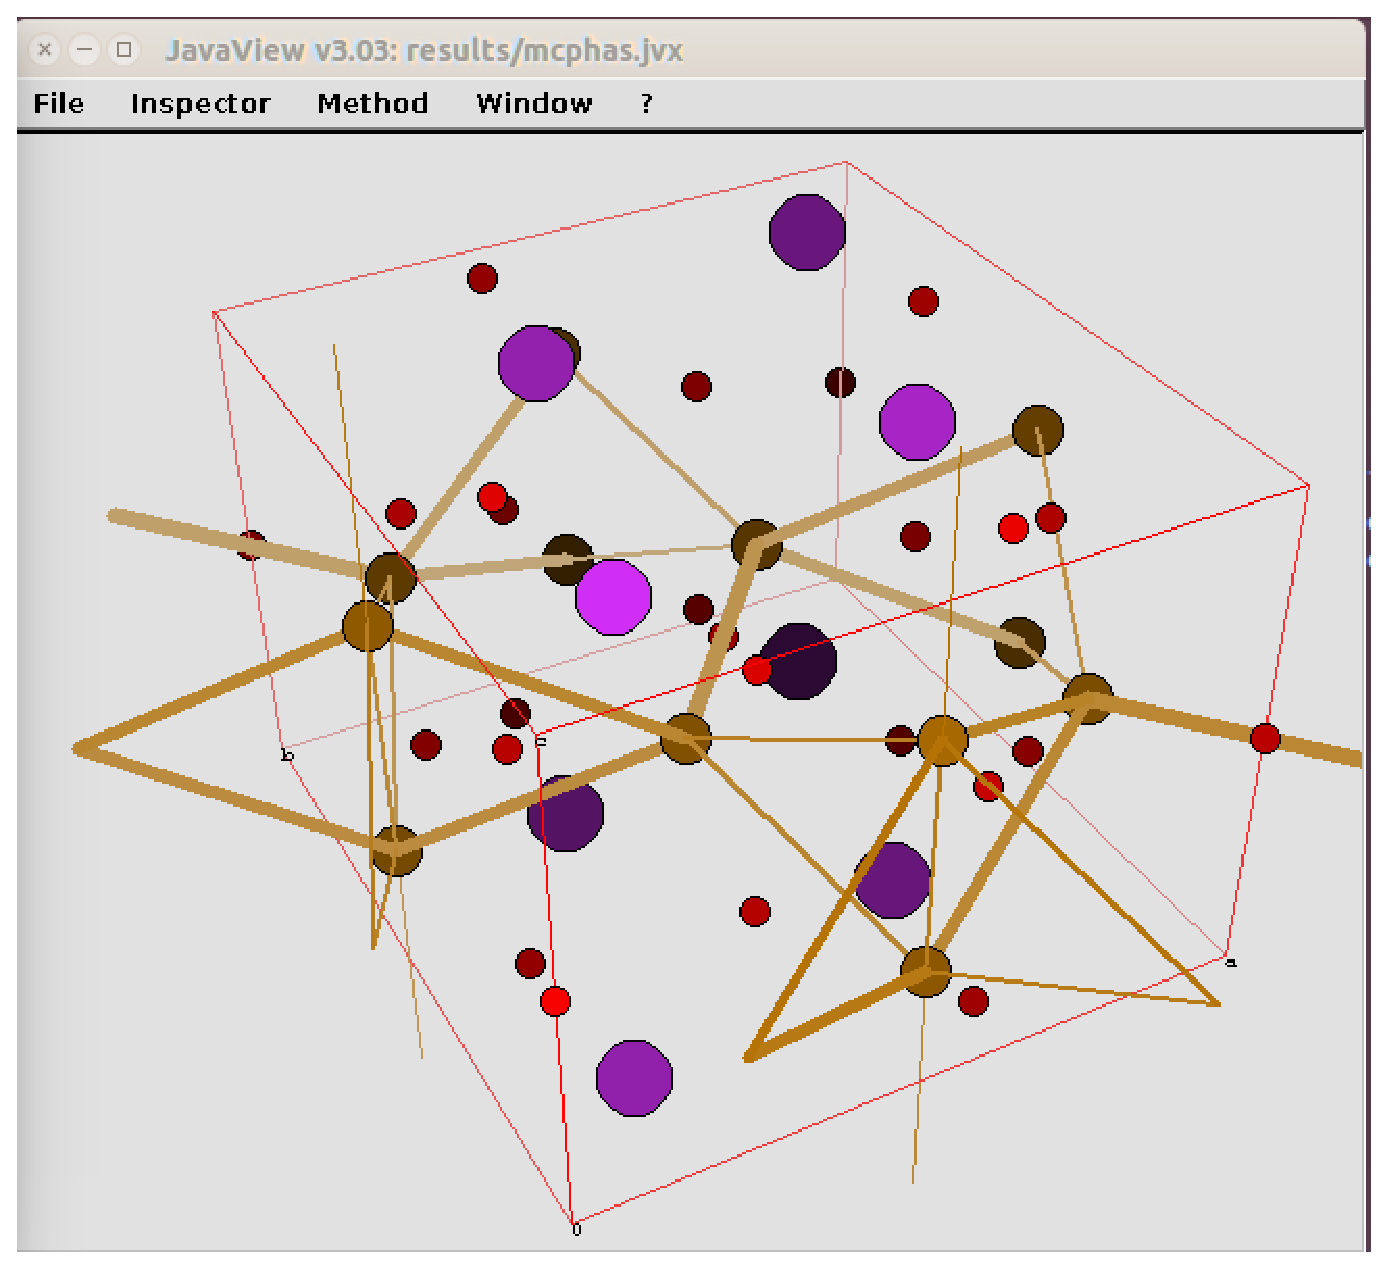
\includegraphics[angle=0, width=0.4\textwidth]{figsrc/mcphas_jvx.eps}
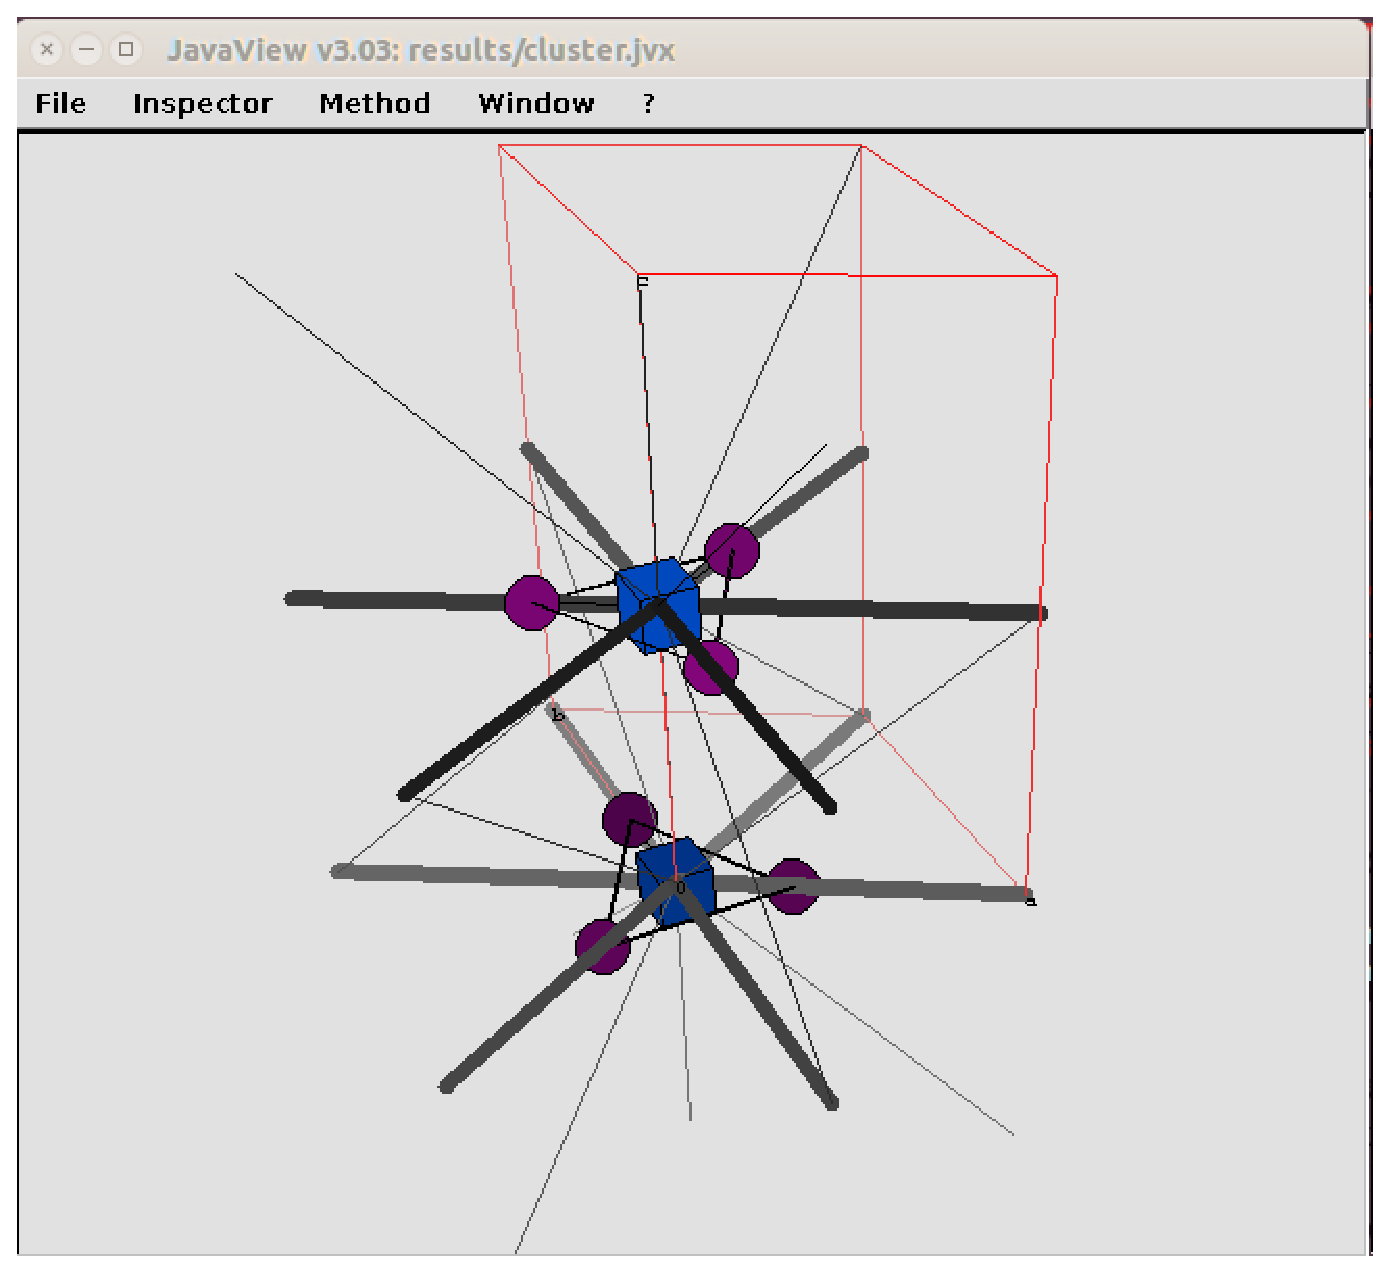
\includegraphics[angle=0, width=0.4\textwidth]{figsrc/trimer_jvx.eps}
\end{center}
\caption{Example of output of mcphas2jvx+JavaView for a normal setup (left, Bi$_2$Fe$_4$O$_9$ with Fe-Fe exchange interactions shown as
lines) and for a cluster setup (right, trimers in LuMnO$_3$ shown as triangles with blue square block indicating trimer centre; intra-trimer
exchange shown as purple lines, inter-cluster exchange as black lines). Linewidths are proportional to the strength of the exchange 
interactions between the linked atoms or clusters.}
\label{mcphas2jvx}
\end{figure}

\item [\prg pointc\index{pointc}{[options]} {ionname$|$sipffile charge\_and\_position$|$file.pos}:]\addcontentsline{toc}{subsubsection}{\prg pointc}
Program to calculate Crystal field Parameters from Point Charges 
\begin{description}
\item [example 1: pointc  Ce3+ 0.2 4 1 5.3]
 ... calculate Blm (Stevens Parameters) and Llm (Wybourne Parameters) for one point 
    charge of +0.2$|e|$ in distance
                 x=4 \AA y=1 \AA z=5.3 \AA from a Ce$^{3+}$ ion. See equation~(\ref{pcmodel}) and
appendix~\ref{cfparconventions} for formulas.
\item [example 2: pointc Ce3+ file.pos]
 ... read several charges+coordinates from file.pos,file format:
      column 1=charge, column 2-4 = x y z coordinate. (note,program {\prg makenn}
      creates useful files for this option from the crystal structure).
\item [example 3: pointc Ce3+ C2.pos 5 6]
 ... same as example 2 but reduced charge model,i.e. B2m calculated, with
     charges in col 1 of C2.pos,B4m and B6m with charges in col 5 and 6, respectively.
Note: if an ion is not implemented, it's parameters can be 
                      entered in a single ion property file and {\prg pointc\index{pointc}} is
                      started as 
\item [example 4: pointc file.sipf 0.2 4 1 5.3 0.1 0.3]
... will use $0.2|e|$ for $B_2^m$, $0.1|e|$ for $B_4^m$, $0.3|e|$ for $B_6^m$.
 ... the first line of the single ion property file.sipf must be
\begin{verbatim}
 #!MODULE=so1ion
\end{verbatim}
The single ion property file must then contain the following
                      information (\# denotes comments):
\begin{verbatim}
 # file.sipf should contain the following information (# denotes comments):
 # the name of the ion
 IONTYPE=Ce3+
 #Stevens parameters (optional, necessary for output of Blm)
 ALPHA=-0.0571429 BETA=0.00634921 GAMMA=0
 # the radial matrix elements RN=<r^N> in units of a0^N (a0=0.5292 A)
 R2=1.309 R4=3.964 R6=23.31
 #optional radial wave function parameters, for transition metal ions the the values
 #are tabulated in Clementi & Roetti Atomic data and nuclear data tables 14 
 #(1974) 177-478, the radial wave function is expanded as
 # R(r)=sum_p Cp r^(Np-1) exp(-XIp r)(2 XIp)^(Np+0.5)/sqrt(2Np!)
 #rare earth:Freeman&Watson PR127(1962)2058,Sovers J.Phys.Chem.Sol.28(1966)1073
 #e.g. Co2+ is isoelectronic to Fe+, looking at page 422
 #of Clemente & Roetti the parameters are 
 N1=3 XI1=4.95296 C1=0.36301 
 N2=3 XI2=12.2963 C2=0.02707 
 N3=3 XI3=7.03565 C3=0.14777
\end{verbatim}
\end{description}

OUTPUT:
\begin{itemize}
\item         {\prg stdout} ... sipf file with CEF pars,radial matrix elements,Stevens factors,
                pointcharges and positions (omit with option -o)
\item         {\prg results\textbackslash pointc.out} ...contains results of convergence when summing up
                 contributions of different neighbours one by one...
\item         {\prg results\textbackslash pointc.Blm} ... Crystal field parameters $B_l^m$ in Stevens Notation
\item         {\prg results\textbackslash pointc.Llm} ... Crystal field parameters $L_l^m$ in Wybourne Notation
\item         {\prg results\textbackslash pointc.dBlm} .. for option -d derivatives $dB_l^m/du$
\item         {\prg results\textbackslash pointc.dLlm} .. for option -d  derivatives $dL_l^m/du$,
                  derivatives are with respect to $u=$neighborposition$(\AA)/a_0$            
\end{itemize}
\item [\prg powdercell2j\index{powdercell2j} file:]\addcontentsline{toc}{subsubsection}{\prg powdercell2j}     used to create mcphas.j type file from %%@
output of powdercell,output is written to mcphas.j.  Example of input file:
\begin{verbatim}
  No   name       crystal coordinates          cartesian coordinates
                 x        y        z           x        y        z
  ------------------------------------------------------------------
  1     Sr1    0.3644   0.0000   0.2500     1.0962  -4.1497  -2.7991
  ...
  \end{verbatim}
\item[\prg radwavfunc\index{radwavfunc} file.sipf:]\addcontentsline{toc}{subsubsection}{\prg radwavfunc} program to evaluate the radial wave function
given by th parametrisation in file.sipf.
\item[\prg reduce\_unitcell\index{reduce\_unitcell} mcphas.j:] \addcontentsline{toc}{subsubsection}{\prg reduce\_unitcell}
                This program checks every atom in the unit cell in file mcphas.j and removes
                any atom, which is connected to another by a lattice vector. Useful for
                going from a description in an extended unit cell to the primitive unit cell.
\begin{description}
\item[Option: -nofcomponents 23] fixes the nofcomponents to 23 by 
                         reducing (removing entries) or increasing (by filling with zeroes) 
                         the exchange parameter tables
\item[Option:  -ni ] forces output without indexchange 
\item[Option: -delatoms 1,2,5,7 ]  instead of removing atoms connected by a lattice vector 
 			remove atoms number 1,2,5 and 7 from the list and also all interactions with those 
\item[Option: -delatoms 1:3+-0.75:4+-0.25,2,5,7]  removes atoms number 1,2,5,7 for atom 1 the interactions
 			 are transferred to 75\% to atom 3 and 25\% to atom 4 and interactions to atoms 3 and 4 are
 			 removed, for 2 5 7 all the interactions with other atoms are removed
\item[Option: -v ] verbose mode
\end{description}
\item [\prg rotateBlm\index{rotateBlm}]\addcontentsline{toc}{subsubsection}{\prg rotateBlm}
  \begin{verbatim}
    Rotates a set of  crystal field  parameters for  Stevens equivalent
    operators by an azimuthal angle fi about the original z axis and
    a polar angle theta about the new y axis. A right hand axis system is assumed
    and a positive rotation is one which advances a right-hand screw in a
    positive direction along the axis.

    The calculations are  done by means of matrix  multiplication based on
    the method of Buckmaster (phys. stat. sol. a, vol 13,  pp 9, 1972) and
    Rudowicz (J. Phys: Solid State Phys., vol 18, pp 1415, 1985).   

    usage: $0 [-h] [--help] 
              [-i input_file] [--input input_file]
	      [-o output_file] [--output output_file]
              [-v] [--verbose] [-th theta] [-fi fi] [CF parameters]

          
     -h          : this (help) message
     -i in_file  : input CF parameters file in cfield or mcphase formats
     -o out_file : output CF parameters file in mcphase format
     -v          : verbose mode. Will print out input parameters as read.
     -th	 : polar angle theta in degrees
     -fi         : azimuthal angle fi in degrees

    if -i is omitted, the program will  assume the input CF parameters are
          given on the command line in the format: Bkq=x.xx,Bkq=x.xx, etc.
          e.g. $0 B20=0.21,B40=0.0005,B60=0.051,B66=0.626
    negative q parameters such as B_2^{-2},  are specified as:  B22S, with 
          an 'S' at the end, as per the McPhase convention.
    you may also  specify the ion type by a dding another  parameter after
          the CF parameters: e.g. $0 B20=0.21,B40=0.5 Pr3+
    if -o is omitted, the program prints the parameters to standard output.
  \end{verbatim}
\item[\prg   setup\_jqfit\index{setup\_jqfit}{[-h]} {[--help]} h k l:]\addcontentsline{toc}{subsubsection}{\prg setupo\_jqfit} program to setup a fit of exchange parameters in order to reproduce an experimental propagation vector.
\begin{verbatim}
     -h          : print help message
      hkl        : Miller indices of propagation vector

    required input files:

    mcphas.j (+ single ion paramter files)
                 :  structural information including all magnetic atoms

    output files:

    mcdisp.par   :  contains propagation vector and list of other hkl to
                    be probed
    mcdisp.mf    :  required input file for mcdisp
    calcsta      :  required input file for simannfit and searchspace
    calcsta.pl.forfit: file with fitparameters for Bethe slater, RKKY fits
    fit.bat      :  batch to start the fit

   
\end{verbatim}

 After running this program you can start immediately a fit of exchange
    parameters. Edit {\prg calcsta.pl.forfit} and {\prg fit.bat} to fine tune the fit 
    according to your needs.
    During fitting a value of sta $< 1$~ indicates, that the maximum of $J(Q)$ is
    at the propagation vector tau. How much it is below one depends on the
    magnitude of $J(Q)$ for the competing wavevectors in the list in{\prg  mcdisp.par}.

\item [\prg setup\_mcdiff\_in\index{setup\_mcdiff\_in}  T Ha Hb Hc:] \addcontentsline{toc}{subsubsection}{\prg setup\_mcdiff\_in}
\item [\prg setup\_mcdiff\_in\index{setup\_mcdiff\_in}  x y:] 
program
 to setup {\prg mcdiff.in} with information on spinconfiguration
                    to be used by program {\prg mcdiff\index{mcdiff}}. Note, you must
                    have done a {\prg mcphas\index{mcphas}} calculation to stabilise
                    a magnetic structure at the desired Temperature/Field.
                  { \prg   setup\_mcdiff\_in} reads the results of this calculation
                    from {\prg results/mcphas.mf} and generates an input file
                    {\prg mcdiff.in}

\begin{verbatim}
     -h          : help  message
      T          : Temperature (K)
      Ha,Hb,Hc   : Magnetic Field (T)
     x,y         : x,y values in phasediagram

    required input files:

    results/mcphas.sps
                 :  result of a mcphas calculation

    optional input files:

    mcdiff.in
                 :  if present experimental parameters (section 1)
                    and nonmagnetic atoms (section 2) are taken from
                    this file

    output files:

    mcdiff.in    :  required input file for mcdiff

    - after running this program you can start mcdiff to do the calculation
      magnetic diffraction pattern
\end{verbatim}
\item [ \prg   setup\_mcdisp\_mf \index{setup\_mcdisp\_mf} T Ha Hb Hc:]\addcontentsline{toc}{subsubsection}{\prg setup\_mcdisp\_mf} 
\item [ \prg   setup\_mcdisp\_mf \index{setup\_mcdisp\_mf} x y:] 

program to setup{\prg mcdisp.mf} with information on meanfields
                    to be used by program {\prg mcdisp\index{mcdisp}}. Note, you must
                    have done a {\prg mcphas\index{mcphas}} calculation to stabilise
                    a magnetic structure at the desired Temperature/Field.
                    {\prg   setup\_mcdisp\_mf} reads the results of this calculation
                    from {\prg  results/mcphas.mf} and puts the meanfields into
                    {\prg mcdisp.mf}.


\begin{verbatim}
     -h          : this (help) message
      T          : Temperature (K)
      Ha,Hb,Hc   : Magnetic Field (T)
      x,y        : x,y values in phasediagram

    required input files:

    results/mcphas.mf
                 :  result of a mcphas calculation

    output files:

    mcdisp.mf    :  required input file for mcdisp

    - after running this program you can start mcdisp to do the calculation
      of dispersion of excitations or diffuse scattering
\end{verbatim}
\item[\prg   setup\_mcphasjforfit\index{setup\_mcphasjforfit}  {[-h]}:]\addcontentsline{toc}{subsubsection}{\prg setup\_mcphasjforfit} program to setup a fit of exchange parameters by   creating mcphas.j.forfit from mcphas.j
                    
\begin{verbatim}
     -h          : print help message

    required input files:

    mcphas.j (+ single ion parameter files)
                 :  structural information including all magnetic atoms

    output files:

    mcphas.j.forfit  : all interaction parameters are substituted
                       with parJxxx[0.0,-1e0,1e0,0,1e-6]

    - after running this program you must setup a file calcsta 
      to calculate the standard deviation and then you can start
      a fit by simannfit or searchspace
\end{verbatim}\index{simannfit}\index{searchspace}
\item [\prg singleion\index{singleion} [options] T[K] Hexta[T] Hextb[T] Hextc[T] Hxc1 Hxc2 Hxc3 ... Hxcnofcomponents]
\addcontentsline{toc}{subsubsection}{\prg singleion}
 single ion  - calculate single ion expectations values $<Ia>, <Ib> $... and transition energies.
 Options may be used to trigger calculation of magnetic Moment and other Quantities.
\begin{verbatim} 
           T    ..... temperature in Kelvin
           Hext ..... external field in Tesla 
           Hxc... exchange (molecular) field in meV   
\end{verbatim}
{\prg singleion} reads {\prg mcphas.j} and the singleion parameter files quoted therein
and calculates energies, eigenstates, expectation values $<I>$ for the given
temperature, external magnetic field Hext and exchange field Hxc (the
interaction constants given in mcphas.j are ignored).

for each single ion property file the following files are generated:
\begin{verbatim}
   results/file.sipf.levels.cef .. energy levels and eigenstates and <I>
   results/file.sipf.trs ......... transition energies,matrix elements
                                   and (powder) neutron intensities
   results/_file.sipf    ......... input parameter files as read and used by singleion 

options: -nt ......... by default only 5 transition energies are output,
                       if you want more, start e.g. with 
                       option -nt 7 to output 7 transition energies
         -pinit 0.1 .. consider only transitions with population of initial state > 0.1
         -ninit 3  ... consider only transitions from the 3 lowest eigenstates
         -maxE 30  ... consider only transitions with energy lower than 30 meV
         -r ion.sipf . do not read mcphas-j but only the single ion
                       parameter file ion.sipf
         -M  ......... calculate expectation values and transition matrix
                       elements for magnetic moment M instead of I
         -MQ 0 0 1 ... instead of <I> calculate expectation values, transition matrix elements
                       for M(Q=(0 0 1)/A), the Fourier Transform  of magnetic moment density M(r)
         -S  ......... calculate expectation values and transition matrix
                       elements for spin S
         -L  ......... calculate expectation values and transition matrix
                       elements for orbital momentum L
         -v       .... verbose, output more information on ongoing calculation
         -Tsteps 10 27 in addition to initial temperature calculate 10 further temperatures
                       until 27K has been reached
         -Hsteps 20 0 0 10 in addition to initial field calculate 20 further external fields
                       until (0 0 10) Tesla has been reached
         -opmat 2 .... output operator matrix number n=2 to results/op.mat
                Operators in output results/op.mat for different values of n:
                n=0                    Hamiltonian
                n=1,...,nofcomponents  operator Matrix In in standard basis
                n=-1,..,-nofomponents  operator Matrix In for Hamiltonian eigenstates basis
                n>nofomponents: all operator Matrices (n=0 to n=nofcomponents) in standard basis
                n<-nofomponents: all operator Matrices (n=0 to n=-nofcomponents) in Hamiltonian eigenstates basis

note: for calculating T or H dependencies you can put single ion in a loop
       and pipe the result into a file

  .... linux:   for B in $(seq 0 0.1 14); do singleion 2 $B 0 0 0 0 0; done > results/fielddep.dat

  .... windows command line: for /L %B in (0,1,14)  do singleion 2 %B 0 0 0 0 0 >> results\fielddep.dat

  .... windows batch file (needed for noninteger numbers):
          @echo off && setlocal ENABLEDELAYEDEXPANSION
          for /L %%I in (0,2,140) do ( set /A W=%%I/10 && set /A "f = %%I %% 10"
          set B=!w!.!f!
          @echo on && singleion 2 0 0 !B! 0 0 0 && @echo off )
          endlocal && @echo on 
...  LOOP linux using perl:
perl -e 'for($T=1;$T<90;$T+=2){system("singleion ".$T." 1 0 0   0 0 0");}' > results/sus1Tesla.clc
 ... LOOP for windows using perl:
perl -e "for($T=1;$T<90;$T+=2){system('singleion '.$T.' 1 0 0   0 0 0');}" > results\sus1Tesla.clc'

\end{verbatim}      

\item [\prg symhmltn:]\addcontentsline{toc}{subsubsection}{\prg symhmltn} Calculates via group theory, the allowed two-ion multipolar exchange terms
between two ions whose center has some particular point symmetry. Syntax is: 
"{\prg symhmltn $\langle$PTGP$\rangle$ $\langle$l$\rangle$}" where {\prg $\langle$PTGP$\rangle$} is 
the name of the point group (both Hermman-Maguin and Schoenflies notation are understood), and 
{\prg $\langle$l$\rangle$} is the integer multipolar order (l=1 for dipolar exchange, l=2 for 
quadrupolar, etc.).
E.g. "{\prg symhmltn Oh 1}" gives the familiar Heisenberg exchange terms. 
See also: {\prg cfsplit} which calculates the multiplicities of the crystal field split levels of a
particular point group.

\end{description} 

\section{Programs for Manipulation of Columns and Lines in Data Files}

Datafiles usually contain columns of numbers, for example:

\begin{verbatim}
# T(K) mu0H(T)  M(mb/T)  [comment lines start with '#' ]
1      1      0.9
2      1      0.6
3      1      0.4
4      1      0.3
5      1      0.25
\end{verbatim}

The following programs manipulate such data files, for example
the program {\prg delcol} deletes a column from a data file,
some general features are:
\begin{itemize}
\item data files are overwritten 
\item multiple files may be handled by one command, e.g. {\prg delcol 4 *.dat} deletes column 4
in all 
files ending with .dat
\item arguments may contain mathematical expressions, e.g. 
\begin{description}
\item{\prg shifttcol 3x2+27 2xx4 data.dat}\addcontentsline{toc}{subsubsection}{\prg shiftcol} \dots adds to each number in column 33 in file data.dat the number $2^4=8$. 
\item{\prg factcol 2 sin(3.1415/2) data.dat}\addcontentsline{toc}{subsubsection}{\prg factcol} \dots multiplies column 2 in file data.dat with   sin(3.1415/2)
,i.e. with 0.999999989
\end{description}
\end{itemize}

\begin{description}
\item [\prg acoscol\index{acoscol} col{[ecolerr]} file:]\addcontentsline{toc}{subsubsection}{\prg acoscol} calculates arccosine of a column arccos(col) 
\item [\prg add\index{add} colx1 coly1{[ecoly1err]} file1 colx2 coly2{[ecoly1err]} file2:] \addcontentsline{toc}{subsubsection}{\prg add}
   program to add functions y1(x1) with (optional) y1err and y2(x2) with (optional y2err)
       taken from data file1 and data file2

\begin{description}
 \item [input:]
 \item[ file1, file2]         filennames
 \item [colx, coly, colyerr]  columns containing x and y=f(x) and yerror values
\item[  output:]
\item[  file1]            contains in coly1=coly1+f2(colx1)
                   and in   coly1err=sqrt[coly1err$^2$+f2err(colx1)$^2$]
                   f2(colx1) is calculated by linear
                   interpolation
                   f2(colx1)=
                   (colx1-colx2(n)*(coly2(n+1)-coly2(n))/(colx2(n+1)-colx2(n))
                   f2err(colx1)=
                   (colx1-colx2(n)*(coly2err(n+1)-coly2err(n))/(colx2(n+1)-colx2(n))
\end{description}
  note:            colx2 has to be sorted in file2
\item [\prg addcol\index{addcol}  colx{[ecolxerr]} coly{[ecolyerr]} file:]\addcontentsline{toc}{subsubsection}{\prg addcol} adds column x and column y of file, result is %%@
stored in col y
Optional - error is added using the error columns colxerr and colyerr
by colyerr=sqrt(colxerr*colxerr+colyerr*colyerr)
\item [\prg asincol\index{asincol} col const file:]\addcontentsline{toc}{subsubsection}{\prg asincol} calculates arcsine of a column arcsine(col) 
\item [\prg atancol\index{atancol} col const file:]\addcontentsline{toc}{subsubsection}{\prg atancol} calculates arctangens of a column %%@
arctan(col) 
\item [\prg average\index{average} {[option]} n file:]\addcontentsline{toc}{subsubsection}{\prg average} program average  used  to 
 reduce the amount of data in a datafile by deleting close data points.
 The program takes sets of n lines in file and  outputs one line instead
of the n lines. By default the the data line in the middle of the n line
block is output. 
 
\begin{description}
 \item [options:]
  \item[-h, -help]
  \item       [-middle]       middle point is taken (default)
  \item       [-first]       first point is taken 
   \item      [-last]        last point is taken 
   \item      [-av]           points are averaged
   \item      [-sum]           points are added
    \item     [-sumcol=12,13,14]  for column 12,13,14 datapoints are added up and the sum is output
    \item     [-median]       median of points is calculated and output
     \item    [-dmin=0.4]    takes instead of n lines a variable number
                         of lines determined by the condition that
                         data in column n is closer than dmin 
\end{description}       

\item [\prg chi2\index{chi2} col1 col2 col3 *.*]\addcontentsline{toc}{subsubsection}{\prg chi2} is used to calculate the 
 chi-squared from 3 columns in a file: if col1, col2 and col3 are calculation, 
 experiment and experimental error, respectively, then
  chisquared is defined as $\chi^2=\frac{1}{n}\sum_{i=1}^n \frac{({\rm col2}_i-{\rm %%@
col1}_i)^2}{{\rm col3_i}^2}$. For each datapoint the program outputs a line
{\em sta=} deviation$^2$  (experimental error)$^2$ to stdout. This may be 
used directly for generating useful input for fitting in {\prg simannfit}\index{simannfit}.
\item [\prg comment l1 l2 file:]\addcontentsline{toc}{subsubsection}{\prg comment} comments all lines from l1 and l2  (with \#) in a file
\item [\prg compare file1 file2:]\addcontentsline{toc}{subsubsection}{\prg compare} used to compare data file1 and data file2
                all columns and rows are compared and a standard deviation
                is calculated according to sum\_i (file1\_i - file2\_i)\^2
                this standard deviation is output to stdout, e.g. as sta=143.3
\item [\prg convolute\index{convolute} c1 c2 file cx cy convfuncfile {[d1 d2 datafile]}:]\addcontentsline{toc}{subsubsection}{\prg convolute} %%@
convolutes data given as column c1 vs column
                       c2 in file (data pairs $x_i,y_i$) with the convolution function given in %%@
column cx vs cy
		        of convfuncfile (function $c(x)$)
		       Range and step width of output file is determined from range and step 
		        of convfuncfile  unless a datafile is given.  Values out of range of convfile are assumed to be zero,
			convfile has to be sorted according to ascending x.
			Formula: $f(x)=\sum_i y_i c(x-x_i)$ , 
		       output is written to stdout. 

                       If a datafile is given, 
		     with data column d1 and d2, the result of the convolution is
		     calculated for x-values of data column d1 and $f(x)$ is compared to
		     data in column d2 - a standard deviation sta is calculated as
		     sum of squared deviations. As output the datafile is given, however with a scaled column
                 d2 and 2 additional columns are added containing the calculated
                 results of the convolution and the original unscaled data.
                 standard deviation, area of curves etc are output to
                 stdout and to environment variables MCPHASE\_STA etc.

                       
\item [\prg convolute2d\index{convolute2d} c1 c2 c3 file cx cy cz convfuncfile minx maxx Nx miny maxy Ny:]\addcontentsline{toc}{subsubsection}{\prg convolute2d} 
convolutes a 2 dimensional function data given as column c3(c1,c2) in file (data tripls $x_i,y_i, z_i$) with the convolution function given in column cx vs cy vs cz
		        of convfuncfile (function $c(x,y)$)
		       Range and number of points of output file is determined from minx maxx Nx and 
                        miny, maxy Ny.
			Formula: $f(x,y)=\sum_i z_i c(x-x_i,y-y_i)$ . In the program the contribution to
                        the sum is evaluated for a discrete triplet cx cy cz of the convolution function, the 
                        resulting x,y will not correspond to a point on the grid defined by minx, max Nx, miny,maxy Ny -
                        therefore the contribution is distributed (according to distance) onto the neighbouring grid
                       points.
		       output is written to stdout. 
\item [\prg coscol\index{coscol} col const file:]\addcontentsline{toc}{subsubsection}{\prg coscol} calculates cosinus of a column cos(col) 
\item [\prg delcol\index{delcol} col file:]\addcontentsline{toc}{subsubsection}{\prg delcol} deletes column col in file
\item [\prg delcols\index{delcols} col n file:]\addcontentsline{toc}{subsubsection}{\prg delcols} deletes column col several (n) times in file
\item [\prg delcomments *.*]\addcontentsline{toc}{subsubsection}{\prg delcomments} removes every comment line (starting with \#) from a file and %%@
prints the removed lines to screen
\item [\prg delline\index{delline} l1 l2 file:]\addcontentsline{toc}{subsubsection}{\prg delline} deletes lines l1 to l2  in file
\item [\prg delnthline n file]\addcontentsline{toc}{subsubsection}{\prg delnthline}  remove every nth line (n$>$2) in file
\item [\prg dif\index{dif} colx coly n *.*:]\addcontentsline{toc}{subsubsection}{\prg dif} used to calculate d(coly)/d(colx) with %%@
differentiation averaging n points
\item [\prg display\index{display} 5{[e7]} 6{[e8]}  ./results/mcdisp.qei {[colx coly file2]}]\addcontentsline{toc}{subsubsection}{\prg display} displays a graphic on screen as xy %%@
graph
with column 5 as x axis and columns 6 as y axis. By default graphic is a line graph.
However, if error columns (in the example x error column is 7 and y error column is 8)
are given, then symbols with x and y error bars are shown. Several files
can be plotted in the same graph by extending the commandline. If the contents of a file
changes, the plot is automatically updated.
\item [\prg displaybubbles\index{displaybubbles}  5 6 8 ./results/mcdisp.qei]\addcontentsline{toc}{subsubsection}{\prg displaybubbles} works similar as %%@
display, however
a third column is given and the radius of the symbols varied according to the data in 
this column.
\item [\prg displaycontour\index{displaycontour} 5 6 8 ./results/mcdisp.dsigma.tot]\addcontentsline{toc}{subsubsection}{\prg displaycontour} produces a %%@
graphical
display\index{display} of a 3 dimensional dataset as a colour and/or contour plot. Here '5 6 8' 
denote the x,y and z column in file {\prg ./results/mcdisp.dsigma.tot}, which should
be plotted. Figure~\ref{ho2ti2o7diffuse} shows an sample output of this program.
\item [\prg displaytext\index{displaytext} ./results/mcphas.hkl]\addcontentsline{toc}{subsubsection}{\prg displaytext} monitors the file mcphas.hkl in %%@
a text window on screen.
\item [\prg displayhtml\index{displayhtml} calc.bat.html]\addcontentsline{toc}{subsubsection}{\prg displayhtml} monitors the file calc.bat.html in 
a text window on screen.
\item [\prg expcol\index{expcol} col const file:]\addcontentsline{toc}{subsubsection}{\prg expcol} calculates exponent of a column exp(col) 
\item [\prg factcol\index{factcol} col{[ecolerr]} const file:]\item [\prg expcol\index{expcol} col const file:]\addcontentsline{toc}{subsubsection}{\prg factcol}
 multiplies col with a constant in file,
a error colmn may be given and is also multiplied by the absvalue of the constant.
\item [\prg fform\index{fform} col1 col2 format file:]\item [\prg expcol\index{expcol} col const file:]\addcontentsline{toc}{subsubsection}{\prg fform }
 reformats numbers in col1 to col2 in file %%@
with
             a number format given by format. Format is a number format string according
             to c conventions, for example 8.4f or 4.4g  ...             
\item [\prg fillcol  col expression *.*\index{fillcol}] \addcontentsline{toc}{subsubsection}{\prg fillcol} used to fill column with numbers in data file
\begin{verbatim}
 col       ....   column
 expression ...   e.g. 'tan(c1x7.52)+c2'
                  here c1,c2,.. refer to column 1,2,...
                  operations are multiplication (x), division(/)
                  addition (+), subtraction(-), power (xx)
                  trigonometric functions tan,cos,sin, asin,atan,acos
                  exp,(natural) log
 *.*       ....   filenname
\end{verbatim}
\item [\prg fitcol coldata prog col parprog1 parprog2 ... {[]} in filename:]\addcontentsline{toc}{subsubsection}{\prg fitcol}
simple fitting program for data in coldata.
\begin{verbatim}
               []=[and prog col parprog1 parprog2 ... [and ...]]

          coldata ...... column number of data column to be fitted
          prog    ...... program name, e.g. shiftcol
          col     ...... column to which prog should be applied
          parprog1 ..... parameter of the program prog, which should be fitted
          filename... filename

    in order to fit data in column coldata, prog is run many times on
    the column col with varying parameter set parprog1 ..., the result
    is scaled to fit best the experimental data. If several programs
    are combined with option 'and' then the best linear combination of the
    results is calculated by linear regression to fit coldata.

    Starting values for the parameters parprog are taken from the
    commandline. initial Stepwidths are chosen 10percent of parameter value, or may
    be given by adding them to the parameter with an 's', e.g. 100.3s0.1
    If a parameter should not be fitted and kept fix, add an 'f', e.g. 100.3f

    output: - files can be found in directory results
            - filename.fit is created with fitted function and parameter values

    examples:
    1) to fit a gaussian to column 2 in datafile expdat (with xvalues in column 1)
    with starting values 132.3, 0.5 and 10 for position, fwhm and area, respectively:

    fitcol 2 gausscol 1 132.3 0.5 10 in exp.dat


    2) to do the same fit but with a background create a column 3, fill it
       with constant values and use echo as a fake column manipulation program
      doing nothing.

   newcol 3 -c 1.0 exp.dat
   fitcol 2 gausscol 1 132.3 0.5 10 and rem 3 in exp.dat

   3) to do the same with a linear background, put into a column 4 the x values

   newcol 4 -c 4.0 exp.dat
   fitcol 2 gausscol 1 132.3 0.5 10 and rem 3 and rem 4 in exp.dat

   4) to fit two gaussians with fixed fwhm and stepping in position initially
    only with 0.1

   fitcol 2 gausscol 1 132.3s0.1 0.5f 10 and  gausscol 1 100.3s0.1 0.5f 10 and rem 3 and rem 4 in exp.dat
\end{verbatim}

\item[\prg gausscol\index{gausscol} col position fwhm area *.*:] \addcontentsline{toc}{subsubsection}{\prg gausscol} calculate a
gaussian from the x values given in column col.

The formula for a gaussian is:
$\sigma={\rm fwhm}/\sqrt{8*log(2)}$,
${\rm gauss}(x)=\frac{{\rm area} exp(-(x-{\rm position})^2/2 \sigma^2)}{\sqrt{2*\pi}\sigma}$

\item[\prg getvalue\index{getvalue} colx coly xvalue dx filename]\addcontentsline{toc}{subsubsection}{\prg getvalue}
program to get the y-value of a function by averaging
 over an interval xvalue+-dx,
 note: colx has to be sorted
\begin{verbatim}
 output: the y-value is written to stdout and environment variable MCPHASE_YVALUE
         1/y-value is written to stdout MCPHASE_YVALUE_INVERSE
         standarddeviation to stdaout and MCPHASE_STA
\end{verbatim}
\item[\prg getvariable\index{getvariable} variablename filename]\addcontentsline{toc}{subsubsection}{\prg getvariable}
 program to get the value of a variable from a file 
  (e.g. somewhere in a file there is 
   a statement T=4.3 and you want to get out this 4.3)
\begin{verbatim}
 output: the variable value is written to stdout and environment variable 
         MCPHASE_GETVARIABLE_VALUE, the name is stored in 
         MCPHASE_GETVARIABLE_NAME
        mind lines starting with # are ignored (unless these start with #!)
\end{verbatim}
\item[\prg histcol\index{histcol} col {[stepwidth|-n steps]} *.*:]\addcontentsline{toc}{subsubsection}{\prg histcol} generates a histogram of
a column in a data file and stores it in histcol.out. stepwidth is the 
stepwidth of the histogram points. Alternatively the number of
steps in the histogram may be given by e.g. {\prg -n 100}.
\item[\prg int\index{int} {[-m] }colx coly *.*:]\addcontentsline{toc}{subsubsection}{\prg int}
 program  to integrate columnx vs columny=f(x), integration is done 
point by point, the result goes to the data file, the total integral 
INT=$\int f(x)dx$ is printed to stdout and set to the 
 environment variable MCPHASE\_INT.
 option -m: n-th moments\index{moments of a distribution} are calculated according to $\mu_1=\int x f(x)dx$/INT, $\mu_n=\int (x-\mu_1)^n f(x)dx$/INT.
The results go to stdout and environment variables MCPHASE\_INT\_MU\_1,
  MCPHASE\_INT\_MU\_2,MCPHASE\_INT\_MU\_3 ... are set.

\item [\prg linreg\index{linreg} col n file:]\addcontentsline{toc}{subsubsection}{\prg linreg} calculates linear regression of n columns in file
\begin{verbatim}
          col     ...... column containing y_k values followed by
          n       ...... n columns containing x_ik (i=1 to n)
	  filename... filename

    the program calculates the linear regression, i.e. the best values
    of coefficients ai such that y_k~sum_i a_i*x_ik for every data line k
    in the file. The n linear regression equations solved to determin a_i
    are (i,j=1 ...n):

     sum_k x_jk y_k = sum_i a_i (sum_k x_ik * x_jk)

   Output: - sdtoud: best coefficients a_i  and standard deviation
             sta=sum_k (y_k-sum_i a_i*x_ik)^2
           - file: new column col+n+1 contining sum_i a_i*x_ik
\end{verbatim}

\item [\prg lorentzcol\index{lorentzcol} col position fwhm area:] \addcontentsline{toc}{subsubsection}{\prg lorentzcol}calculate a lorentzian from
a column with x values, the formula for a Lorentz curve is: 
${\rm lorentz}(x)=\frac{1.0}{\pi{\rm fwhm}(1.0+(x-{\rm position})^2/fwhm^2)}$
\item [\prg multcol\index{multcol}  colx coly file:]\addcontentsline{toc}{subsubsection}{\prg multcol} multiplies column x and column y of file, %%@
result is stored in col y
\item [\prg newcol\index{newcol} col {[options]} file:]\addcontentsline{toc}{subsubsection}{\prg newcol} creates a new column col in file containing the line numbe. option: -c 12.3  ... instead of line number put constant 12.3 into the new column
\item [\prg newcols\index{newcols} col n {[options]} file:]\addcontentsline{toc}{subsubsection}{\prg newcols} creates n new columns from column col
 in file. New columns are inserted after column col and contain the same data as column col.
 options: -c 12.3 ...  put constant 12.3 into the new columns, -n ... put line number into the new column.
\item [\prg newline\index{newline} n text file:]\addcontentsline{toc}{subsubsection}{\prg newline} creates a new line number n  in file containing %%@
the text 
\item [\prg potcol\index{potcol} col const file:]\addcontentsline{toc}{subsubsection}{\prg potcol}  col=col$^{\rm const}$ in file
\item [\prg range\index{range} col min max file:]\addcontentsline{toc}{subsubsection}{\prg range} deletes (comments out) all data points outside %%@
min max in column  col of
                       file file (remember to store your full data set in some other
		       file before using this command), \# is used to comment lines
\item[\prg rotate\index{rotate} xcol ycol angle file:]\addcontentsline{toc}{subsubsection}{\prg rotate}
program rotate  used to rotate coordinate axes,
 xcol,yxol=columns containing x and y , 
 angle=angle $\alpha$ of rotation around z.
 
 The rotation is done using the following formula:
\begin{eqnarray}
 x'&= &\cos(\alpha)*x+\sin(\alpha)*y \nonumber \\
 y'&=&-\sin(\alpha)*x+\cos(\alpha)*y
\end{eqnarray}
\item [\prg rpvalue\index{rpvalue} colx coly  *.*:]\addcontentsline{toc}{subsubsection}{\prg rpvalue}  program rpvalue\index{rpvalue}  used to %%@
calculate 
                       the $R_p$-value from columns number colx and coly 
		       in a file *.*. The $R_p$-value is defined as
		       \begin{equation}
		       R_p= 100*\frac{\sum_{i=1}^{N} |(x(i)-y(i)|}{\sum_{i=1}^{N}|x(i)|}
		       \end{equation}
                       $N$ denotes the number of data points in the file.
\item [\prg setvalue\index{setvalue} row column text files:]\addcontentsline{toc}{subsubsection}{\prg setvalue} sets the numerical value in a specified position of a data file.

\begin{verbatim}
     row         : row number
     column    : column number
     number   : text to be placed in file at this position
     files         : one or more filenames

    example: $0 4 5 3.142 data.dat
             replaces the number in row 4 and column 5 by 3.142 in file data.dat
\end{verbatim}
\item [\prg shiftcol\index{shiftcol} col const *.*:]\addcontentsline{toc}{subsubsection}{\prg shiftcol} used to add a constant (const) to a column %%@
(number col) in file(s) *.*
\item [\prg sincol\index{sincol} col const file:]\addcontentsline{toc}{subsubsection}{\prg sincol} calculates sinus of a column sin(col) 
\item [\prg sumcol\index{sumcol} col *.*]\addcontentsline{toc}{subsubsection}{\prg sumcol} prints to stdout number of lines, sum of squares, sum %%@
of absolute values of column col in file *.*
\item [\prg swapcol\index{swapcol} colx coly file:]\addcontentsline{toc}{subsubsection}{\prg swapcol} swaps column x and column y of file
\item [\prg tancol\index{tancol} col file:]\addcontentsline{toc}{subsubsection}{\prg tancol} calculates tangens of a column tan(col)
\item [\prg tanhcol\index{tanhcol} col file:]\addcontentsline{toc}{subsubsection}{\prg tanhcol} calculates tangens-hyperbolicus of a column tanh(col)
\item [\prg uvw2fwhm\index{uvw2fwhm} u v w col *.*:]\addcontentsline{toc}{subsubsection}{\prg uvw2fwhm} used to calculate the full
                   width half maximum from
                   2theta in degree according to fullprofs u,v,w parameters ...
                  The column col in file *.* must contain 2theta scattering angle
                 values and is overwritten with the fwhm as calculated by
                  \begin{equation}
                     {\rm  fwhm }= \sqrt {u \tan^2(\theta) + v \tan(\theta) + w}
                \end{equation}
\item [\prg zshift\index{zshift} constx colx coly *.*:]\addcontentsline{toc}{subsubsection}{\prg zshift} shifts colx by a constant such that it %%@
is zero at a specified value constx of colx. 
\end{description}

\section{Programs of General Interest}

\begin{description}
\item [\prg beep\index{beep}:]\addcontentsline{toc}{subsubsection}{\prg beep} just make a beep\index{beep} to signal attention 
\item [\prg export\index{export} A=23.5-7/2.6e-23*\%B\%]\addcontentsline{toc}{subsubsection}{\prg export} program for windows to allow for
simple math operations. Linux users can use some linux syntax such as 
{\prg \begin{verbatim}export A= $(echo 23.5-7/2.6e-23*$B | bc -l )\end{verbatim}}.
\item [\prg gauss\index{gauss} fwhm stp min max:]\addcontentsline{toc}{subsubsection}{\prg gauss} calculate a gaussian, output goes to console %%@
(stdout), the formula for a gaussian is:
$\sigma={\rm fwhm}/\sqrt{8*log(2)}$,
${\rm gauss}(x)=\frac{exp(-x^2/2 \sigma^2)}{\sqrt{2*\pi}\sigma}$
\item [\prg gauss2d\index{gauss2d} fwhm1 fwhm2 theta  stpx minx maxx stpy miny maxy:]\addcontentsline{toc}{subsubsection}{\prg gauss2d} calculate a 2 dimensional gaussian, output goes to console %%@
(stdout), the formula for a two dimensional gaussian is:
$\sigma={\rm fwhm}/\sqrt{8*log(2)}$,
${\rm gauss}(x,y)=\frac{exp(-u_1^2/2 \sigma_1^2)}{\sqrt{2*\pi}\sigma_1}\frac{exp(-u_2^2/2 \sigma_2^2)}{\sqrt{2*\pi}\sigma_2}$ with $u_1=x cos(\theta)-ysin(\theta)$ and $u_2=y cos(\theta)+xsin(\theta)$,
$\theta$ is the rotation angle in degree.
\item [\prg lorentz\index{lorentz} fwhm stp min max:]\addcontentsline{toc}{subsubsection}{\prg lorentz} calculate a lorentzian, output goes to %%@
console (stdout)the formula for a Lorentz curve is: 
${\rm lorentz}(x)=\frac{1.0}{\pi{\rm fwhm}(1.0+x^2/fwhm^2)}$
\item [\prg plotbook *.ps:]\addcontentsline{toc}{subsubsection}{\prg plotbook} program plotbook to arrange many (single side) ps-images to one %%@
booklet (needs: latex, pstops,ghostscript, perl)
\item [\prg script2html\index{script2html} calc1.bat calc2.bat ...]\addcontentsline{toc}{subsubsection}{\prg script2html} This program creates a html file from scripts containing just the text
 in the scripts.
\begin{verbatim}
 input: calc1.bat, calc2.bat ...    scripts (bat files)
                                   (must be located in the current directory)
 output: stdout      ...........   html file created from the scripts
                                   (use ">" to pipe into file)
 example:

 script2html calc.bat notes.txt > report.html

 [creates the html file report.html from files calc.bat and notes.txt]
\end{verbatim}
\item [\prg setvariable\index{setvariable} varname value *.*:]\addcontentsline{toc}{subsubsection}{\prg setvariable}
sets a variable in a file, e.g. {\prg setvariable T 20 Co.sipf} replaces
T=15 by T=20 in file {\prg Co.sipf}.
\item [\prg substitute\index{substitute} {[option]} oldtext newtext *.*:]\addcontentsline{toc}{subsubsection}{\prg substitute} replaces every instance of %%@
oldtext with newtext in file(s) *.*. Option {\prg -f} substitutes only the first occurence, 
{\prg -n 13} substitutes only the 13th occurence of the oldtext.
\end{description}


